\chapter{Gamma detection testing}

The purpose of this experiment is to determine the necessary conditions under which the gamma spectroscopy with selected photodiodes can be performed and find out whether the photodiodes are even capable of detecting gamma rays since the purpose of some them is not defined as a detector of gamma rays. The determination of detection efficiency is precisely done in following chapters for selected photodiodes. 
\par
For the very first test of photodiodes we assembled a spectrometric setup from ORTEC modules including preamplifier ORTEC142A, shaping amplifier 575A and high voltage source inside the ORTEC minibin. The pulses were captured by ORTEC MCA connected to PC running the MAESTRO Multichannel Analyzer Emulation Software \cite{maestro}. 


\begin{figure}[H]
 \centering
 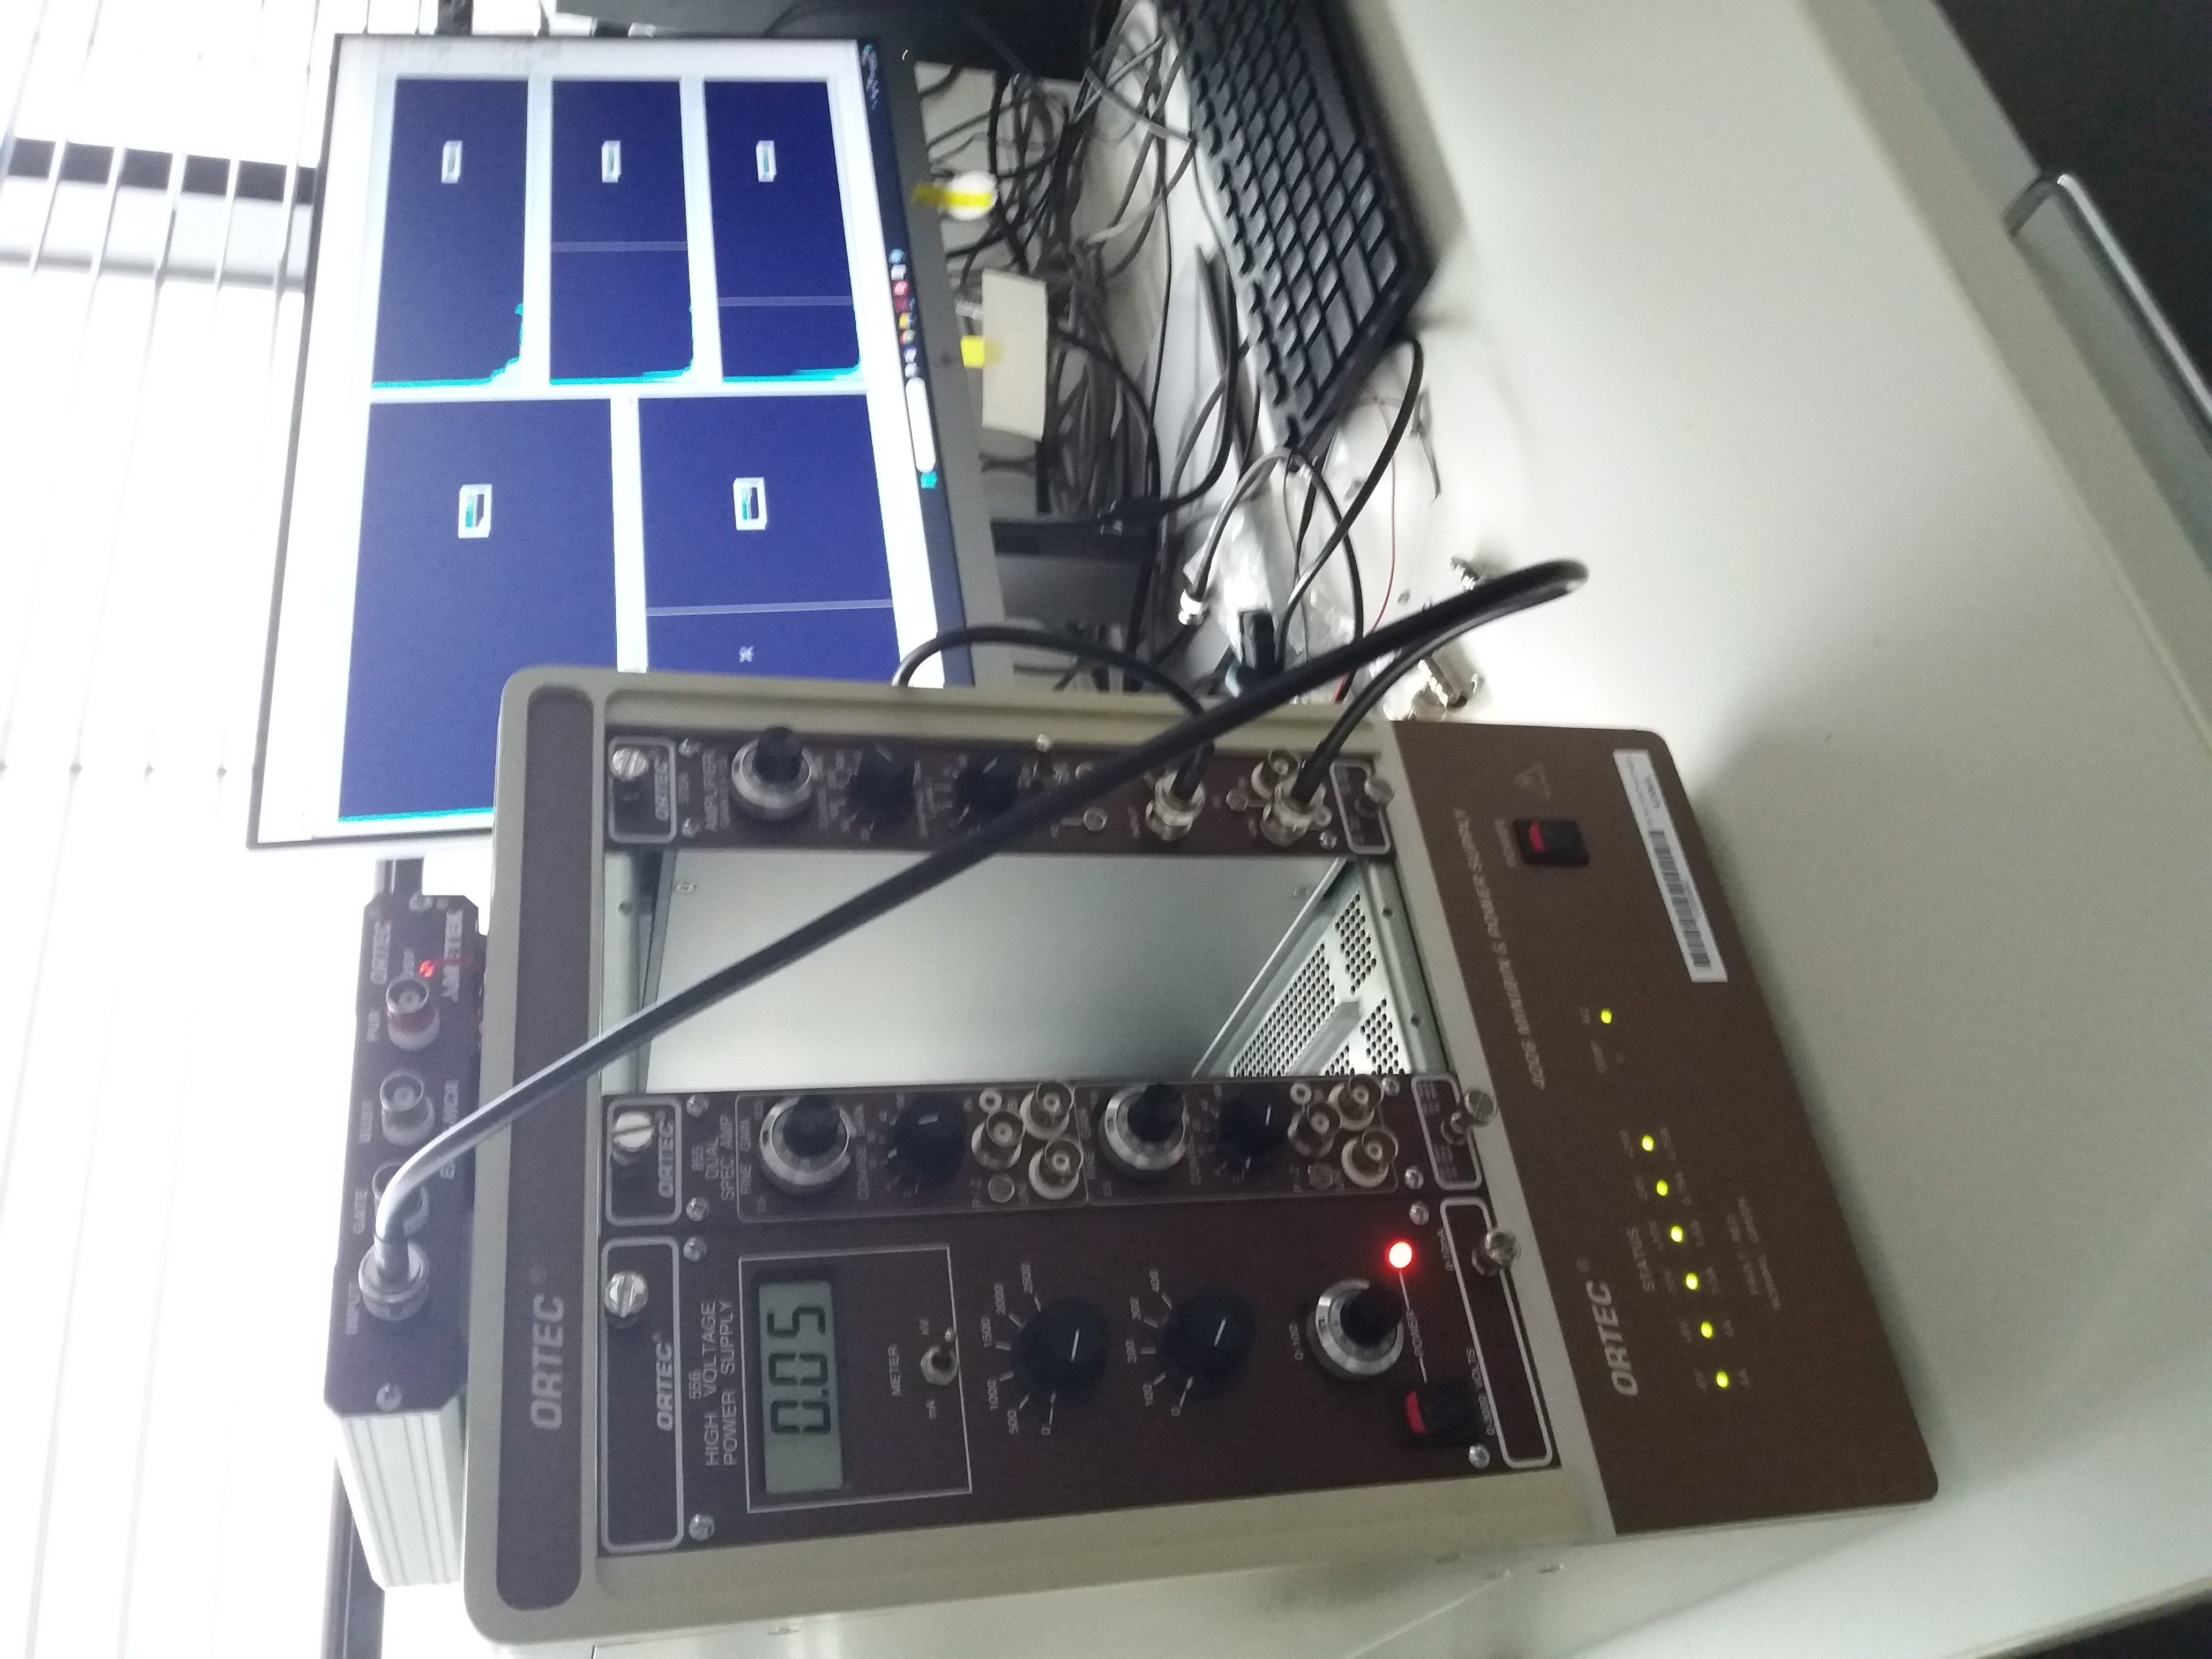
\includegraphics[scale=0.09, angle = 270]{./pictures/ORTECbin.jpg}
 \caption{ORTEC minibin with MCA connected to PC.}
 \label{minibin}
 
\end{figure}
\par
As radiation source we use $^{57}$Co 50 mCi Mössbauer source from 2016 and thus it was necessary to cover the part with radiation source with lead shielding blocks.



\begin{figure}[H]
 \centering
 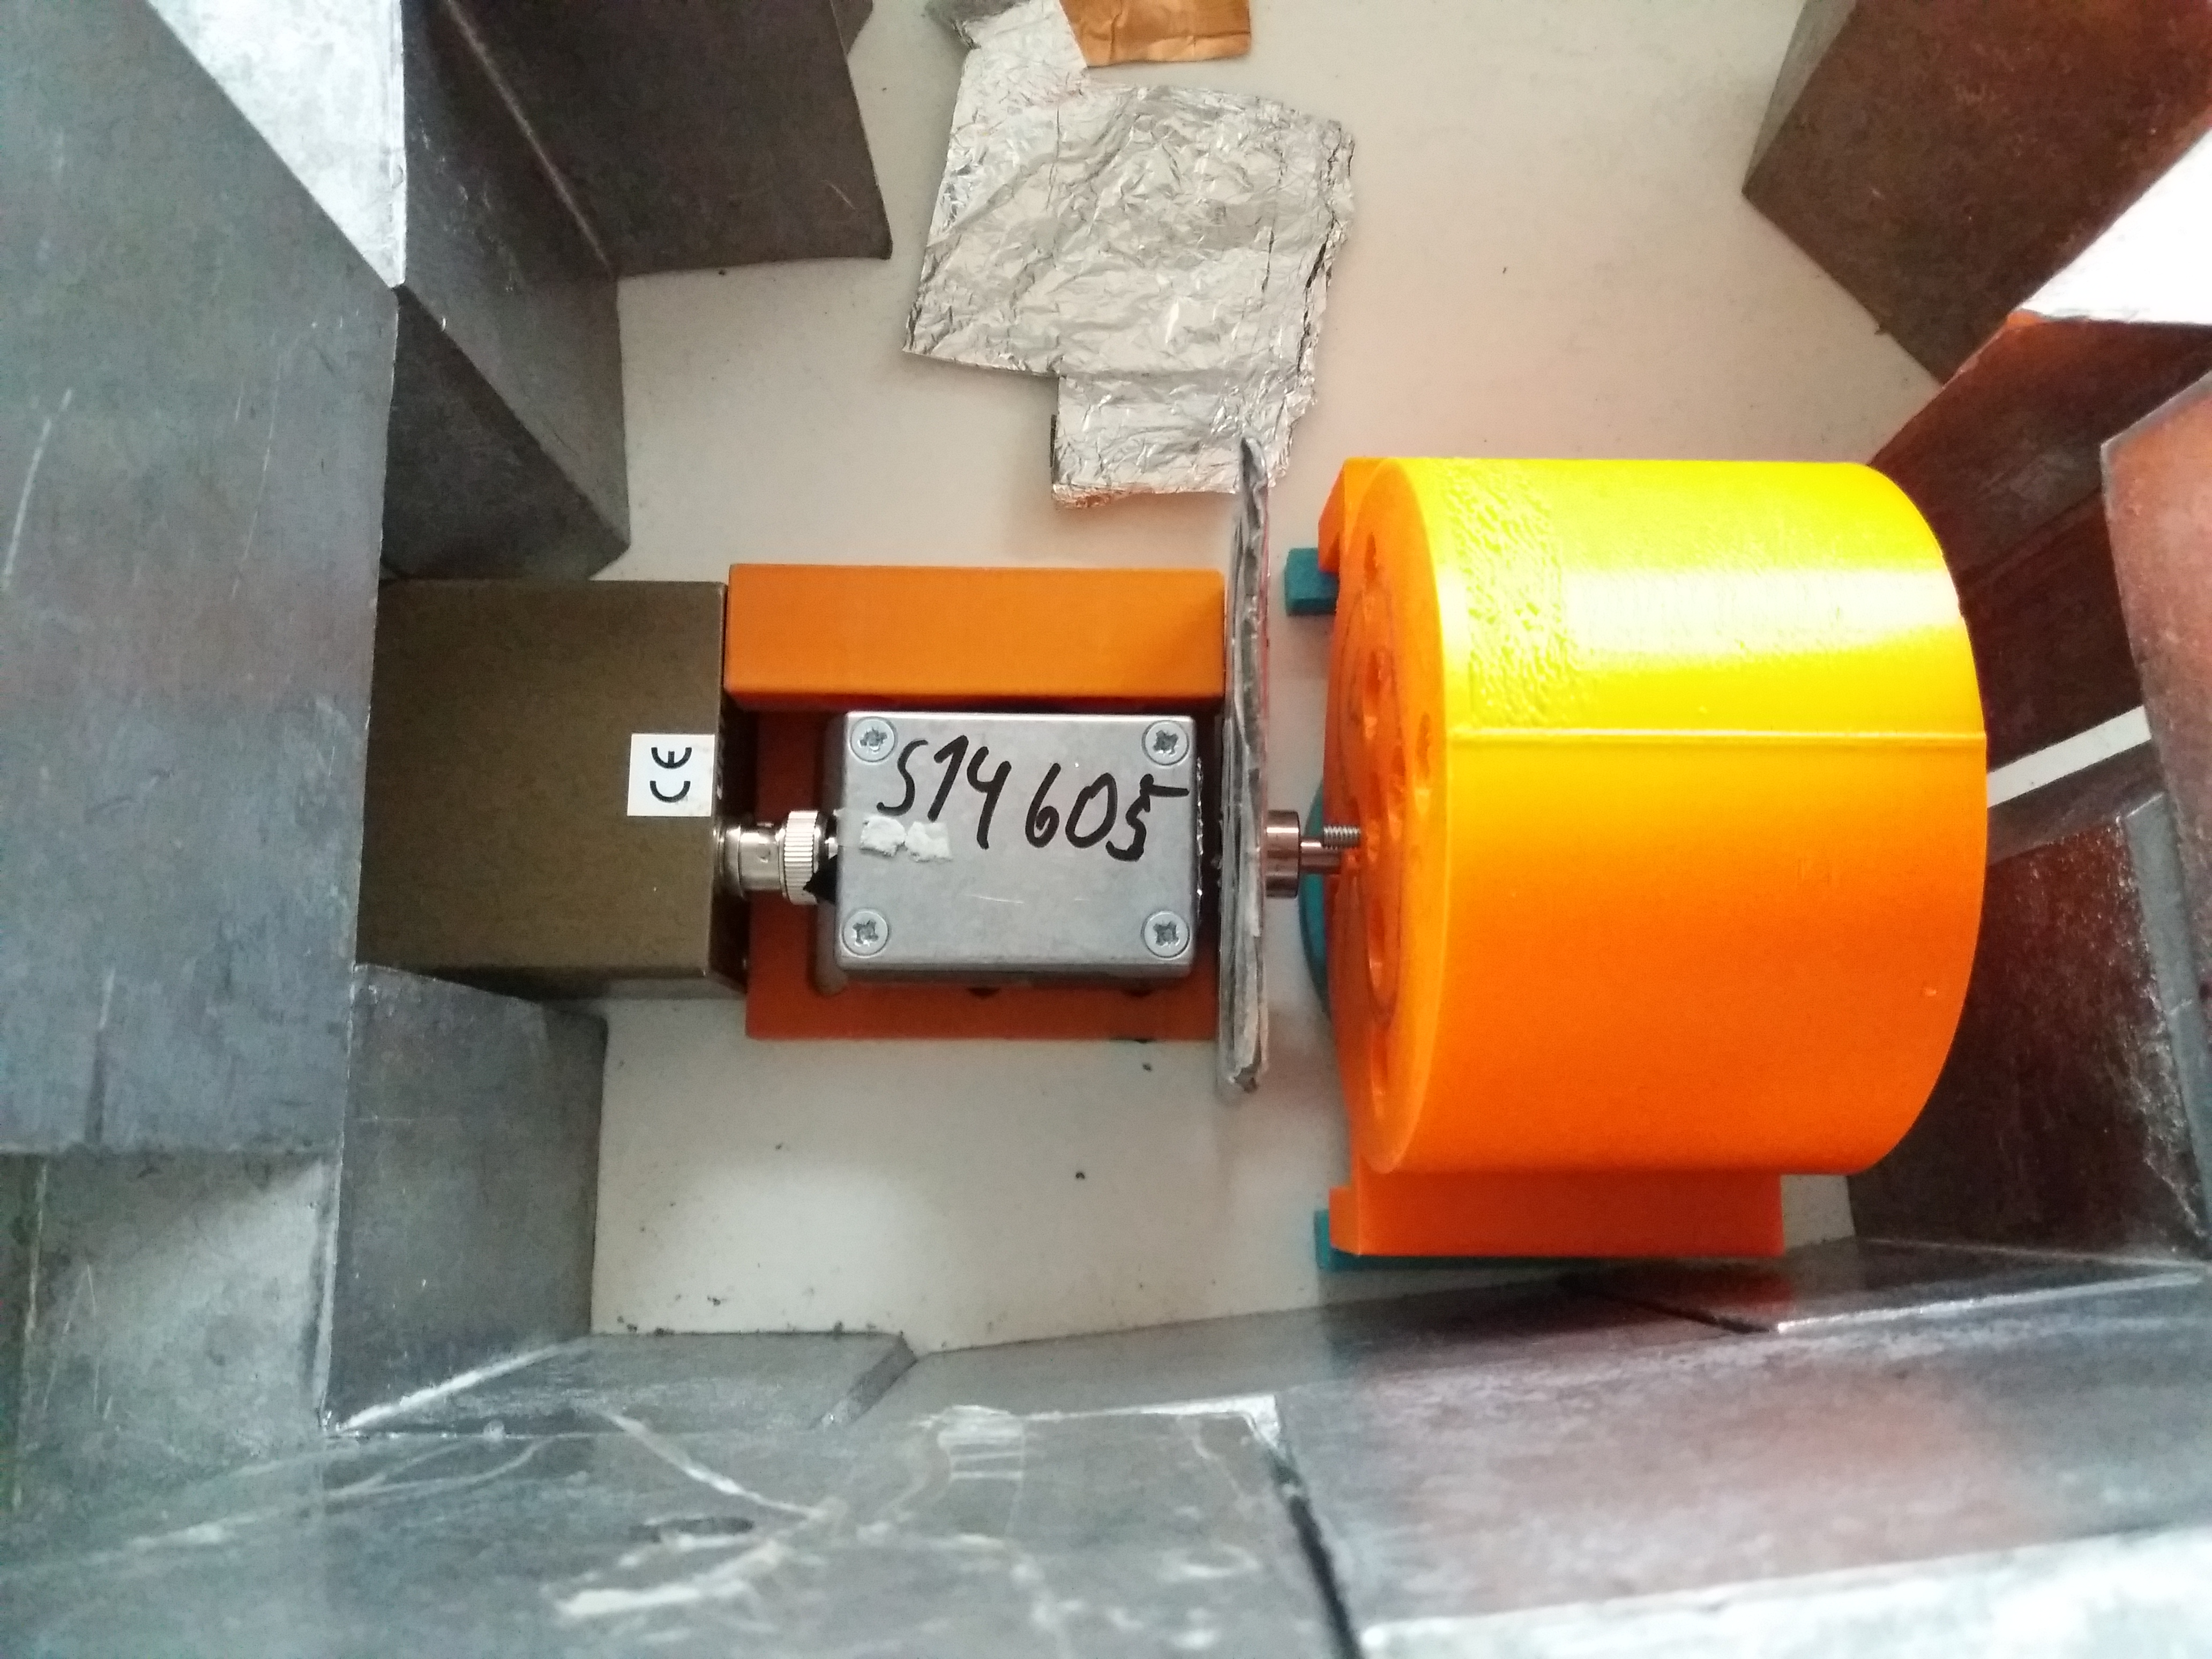
\includegraphics[scale=0.09, angle = 0]{./pictures/ORTECsetup.jpg}
 \caption{PIN diode inside the shielding crate connected to the preamplifier to measure the $^{57}$Co source with filter.}
 \label{setup}
 
\end{figure}


\section{Noise and its reduction}
When performing gamma spectroscopy measurements, the energy spectra are affected by noise. In order to reduce noise as much as possible, two approaches were tested - shielding the detector by various ways and cooling to temperatures near 0 $\circ$C.
\subsection{Electromagnetic noise reduction}
Photodiodes have to be sufficiently electromagnetically shielded and their distance to the preamplifier input should be as short as possible. Using the diodes with poor shielding leads into high levels of electromagnetic noise, which make mayor part of energetic spectra unobservable.
\par
On the behalf of many tests it was proven that the best way to shield the photodiode is to put it into the aluminium crate (see \ref{crate}). This crate has to be small as possible and has to be connected to the grounding potential. However, the front side of the crate has to be open to allow the sufficient transmission of gamma photons to the detector. A drilled hole covered by a thin aluminium foil has sufficient gamma transmission parameters as well as electromagnetic shielding parameters.

\begin{figure}[H]
 \centering
 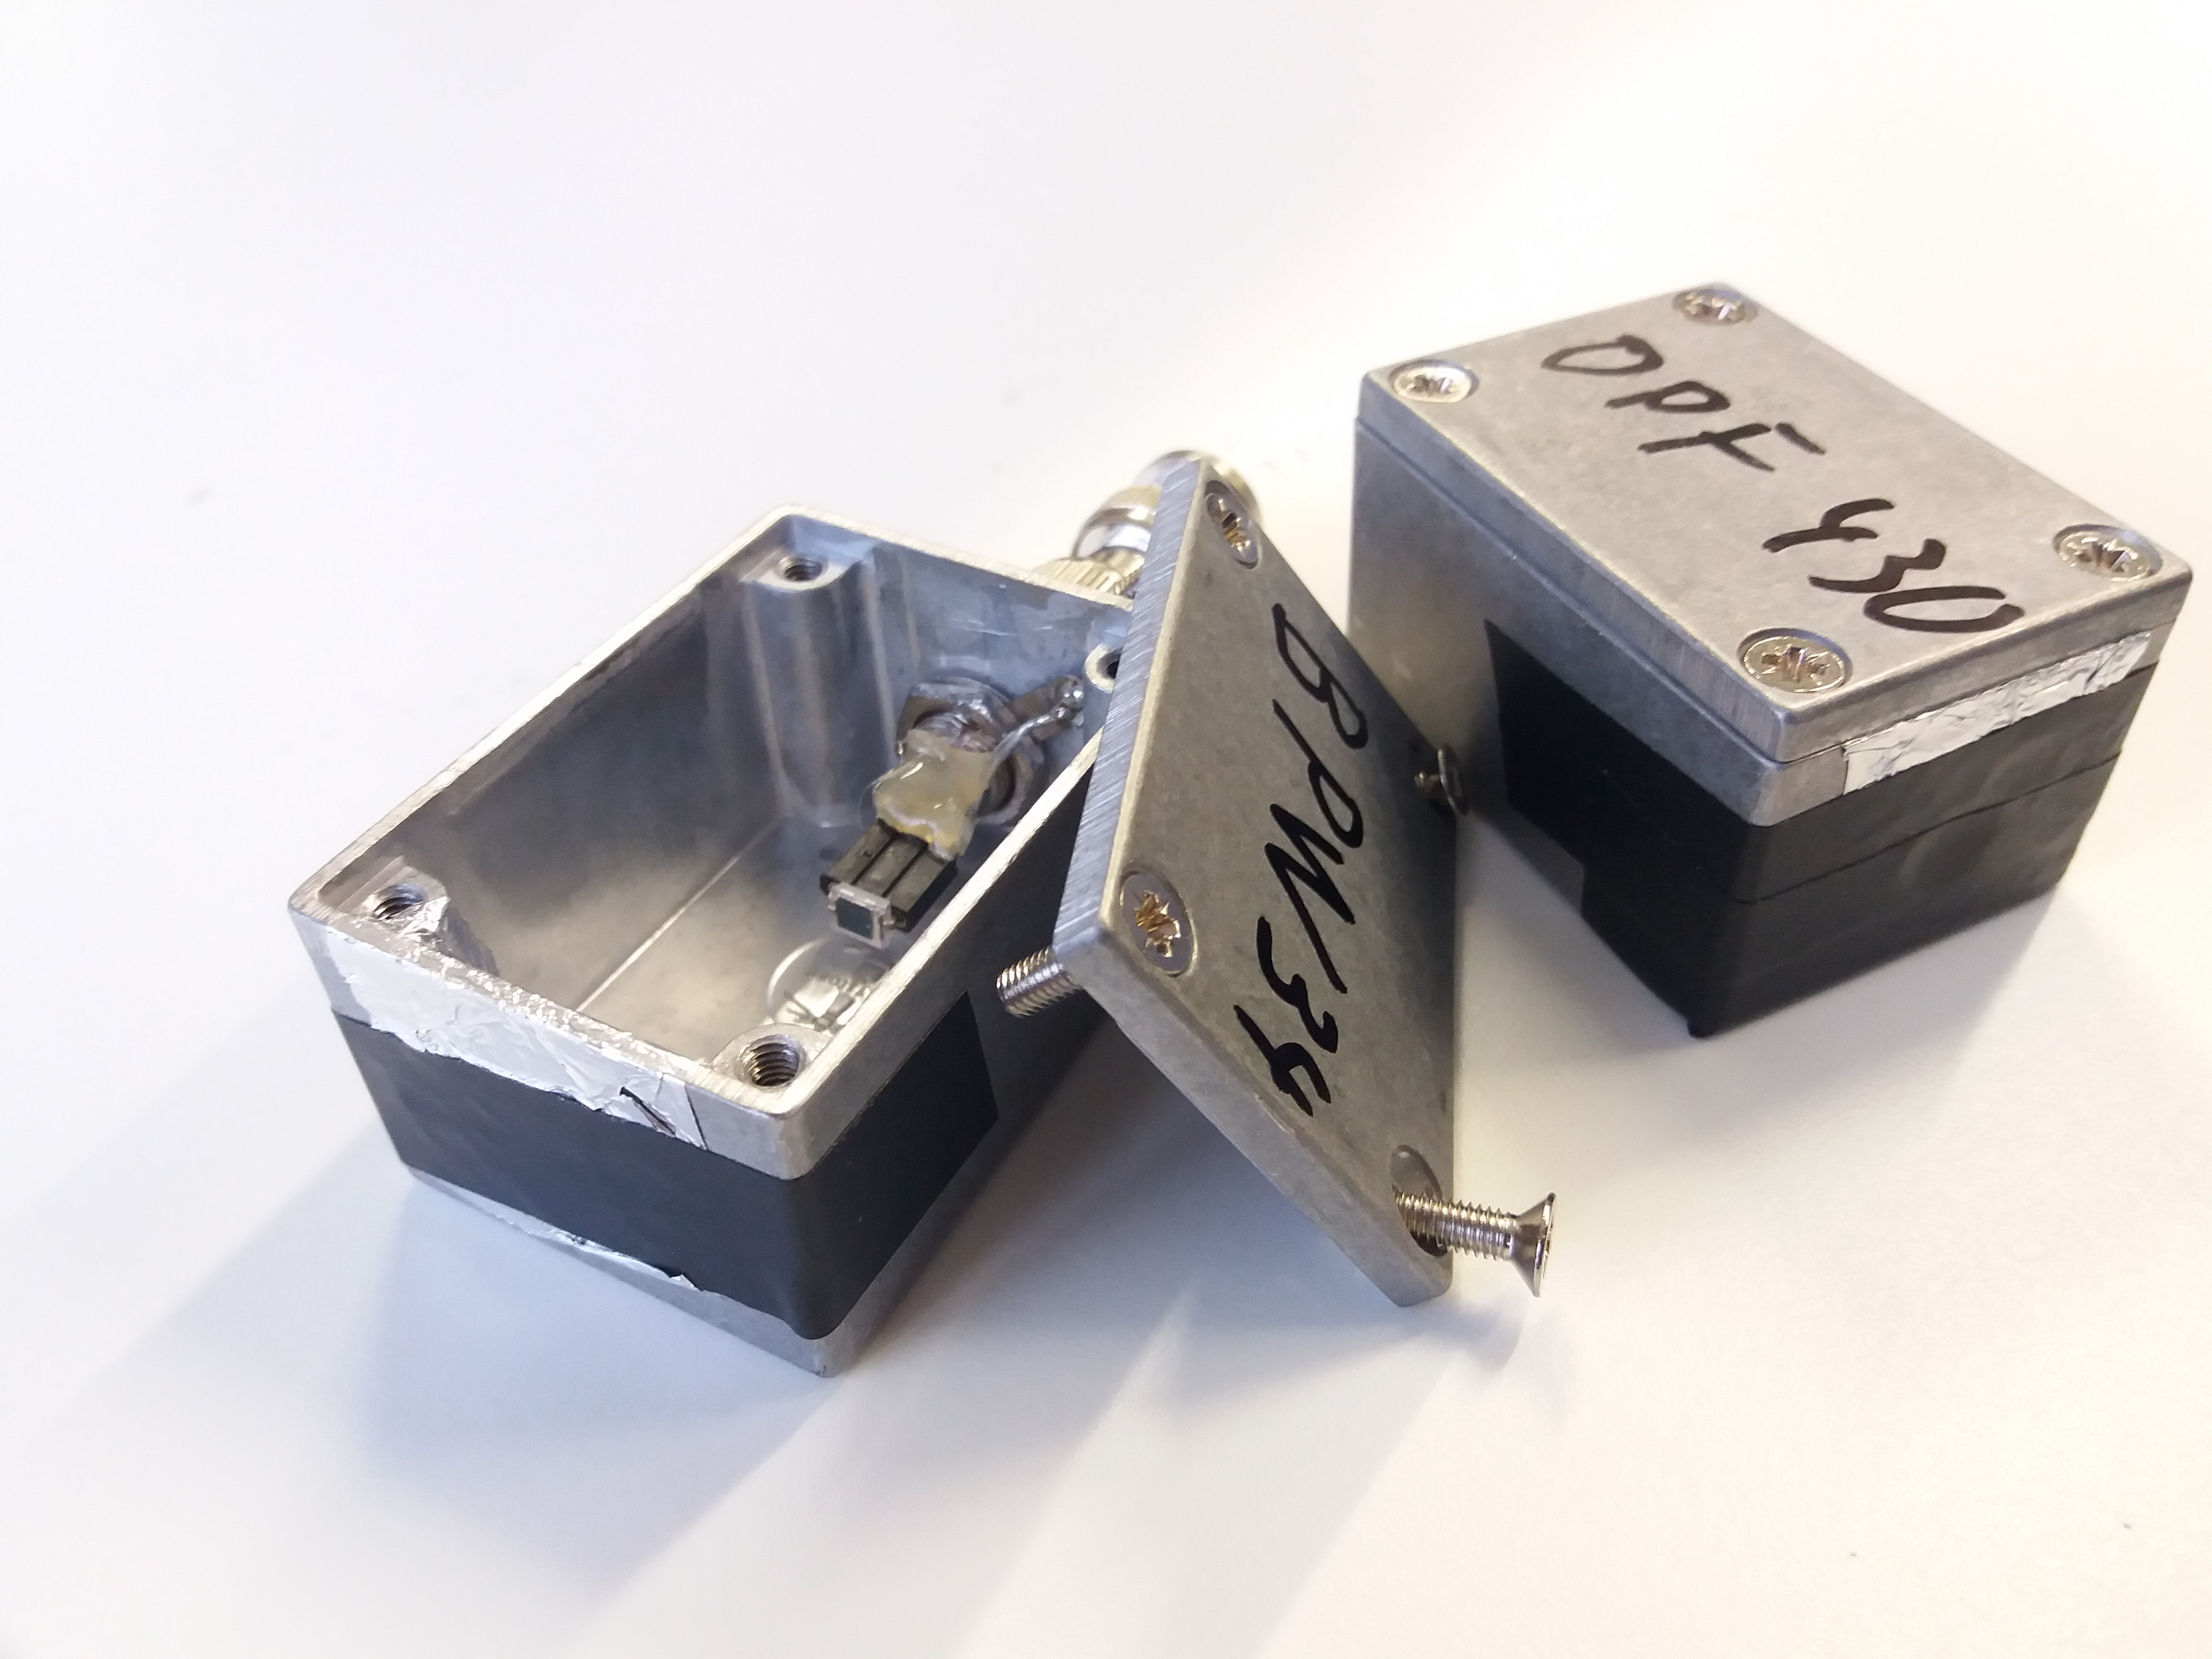
\includegraphics[scale=0.09, angle = 0]{./pictures/ShieldCrate.jpg}
 \caption{Photodiode inside aluminium shielding crates.}
 \label{crate}
 
\end{figure}


\begin{figure}[H]
 \centering
 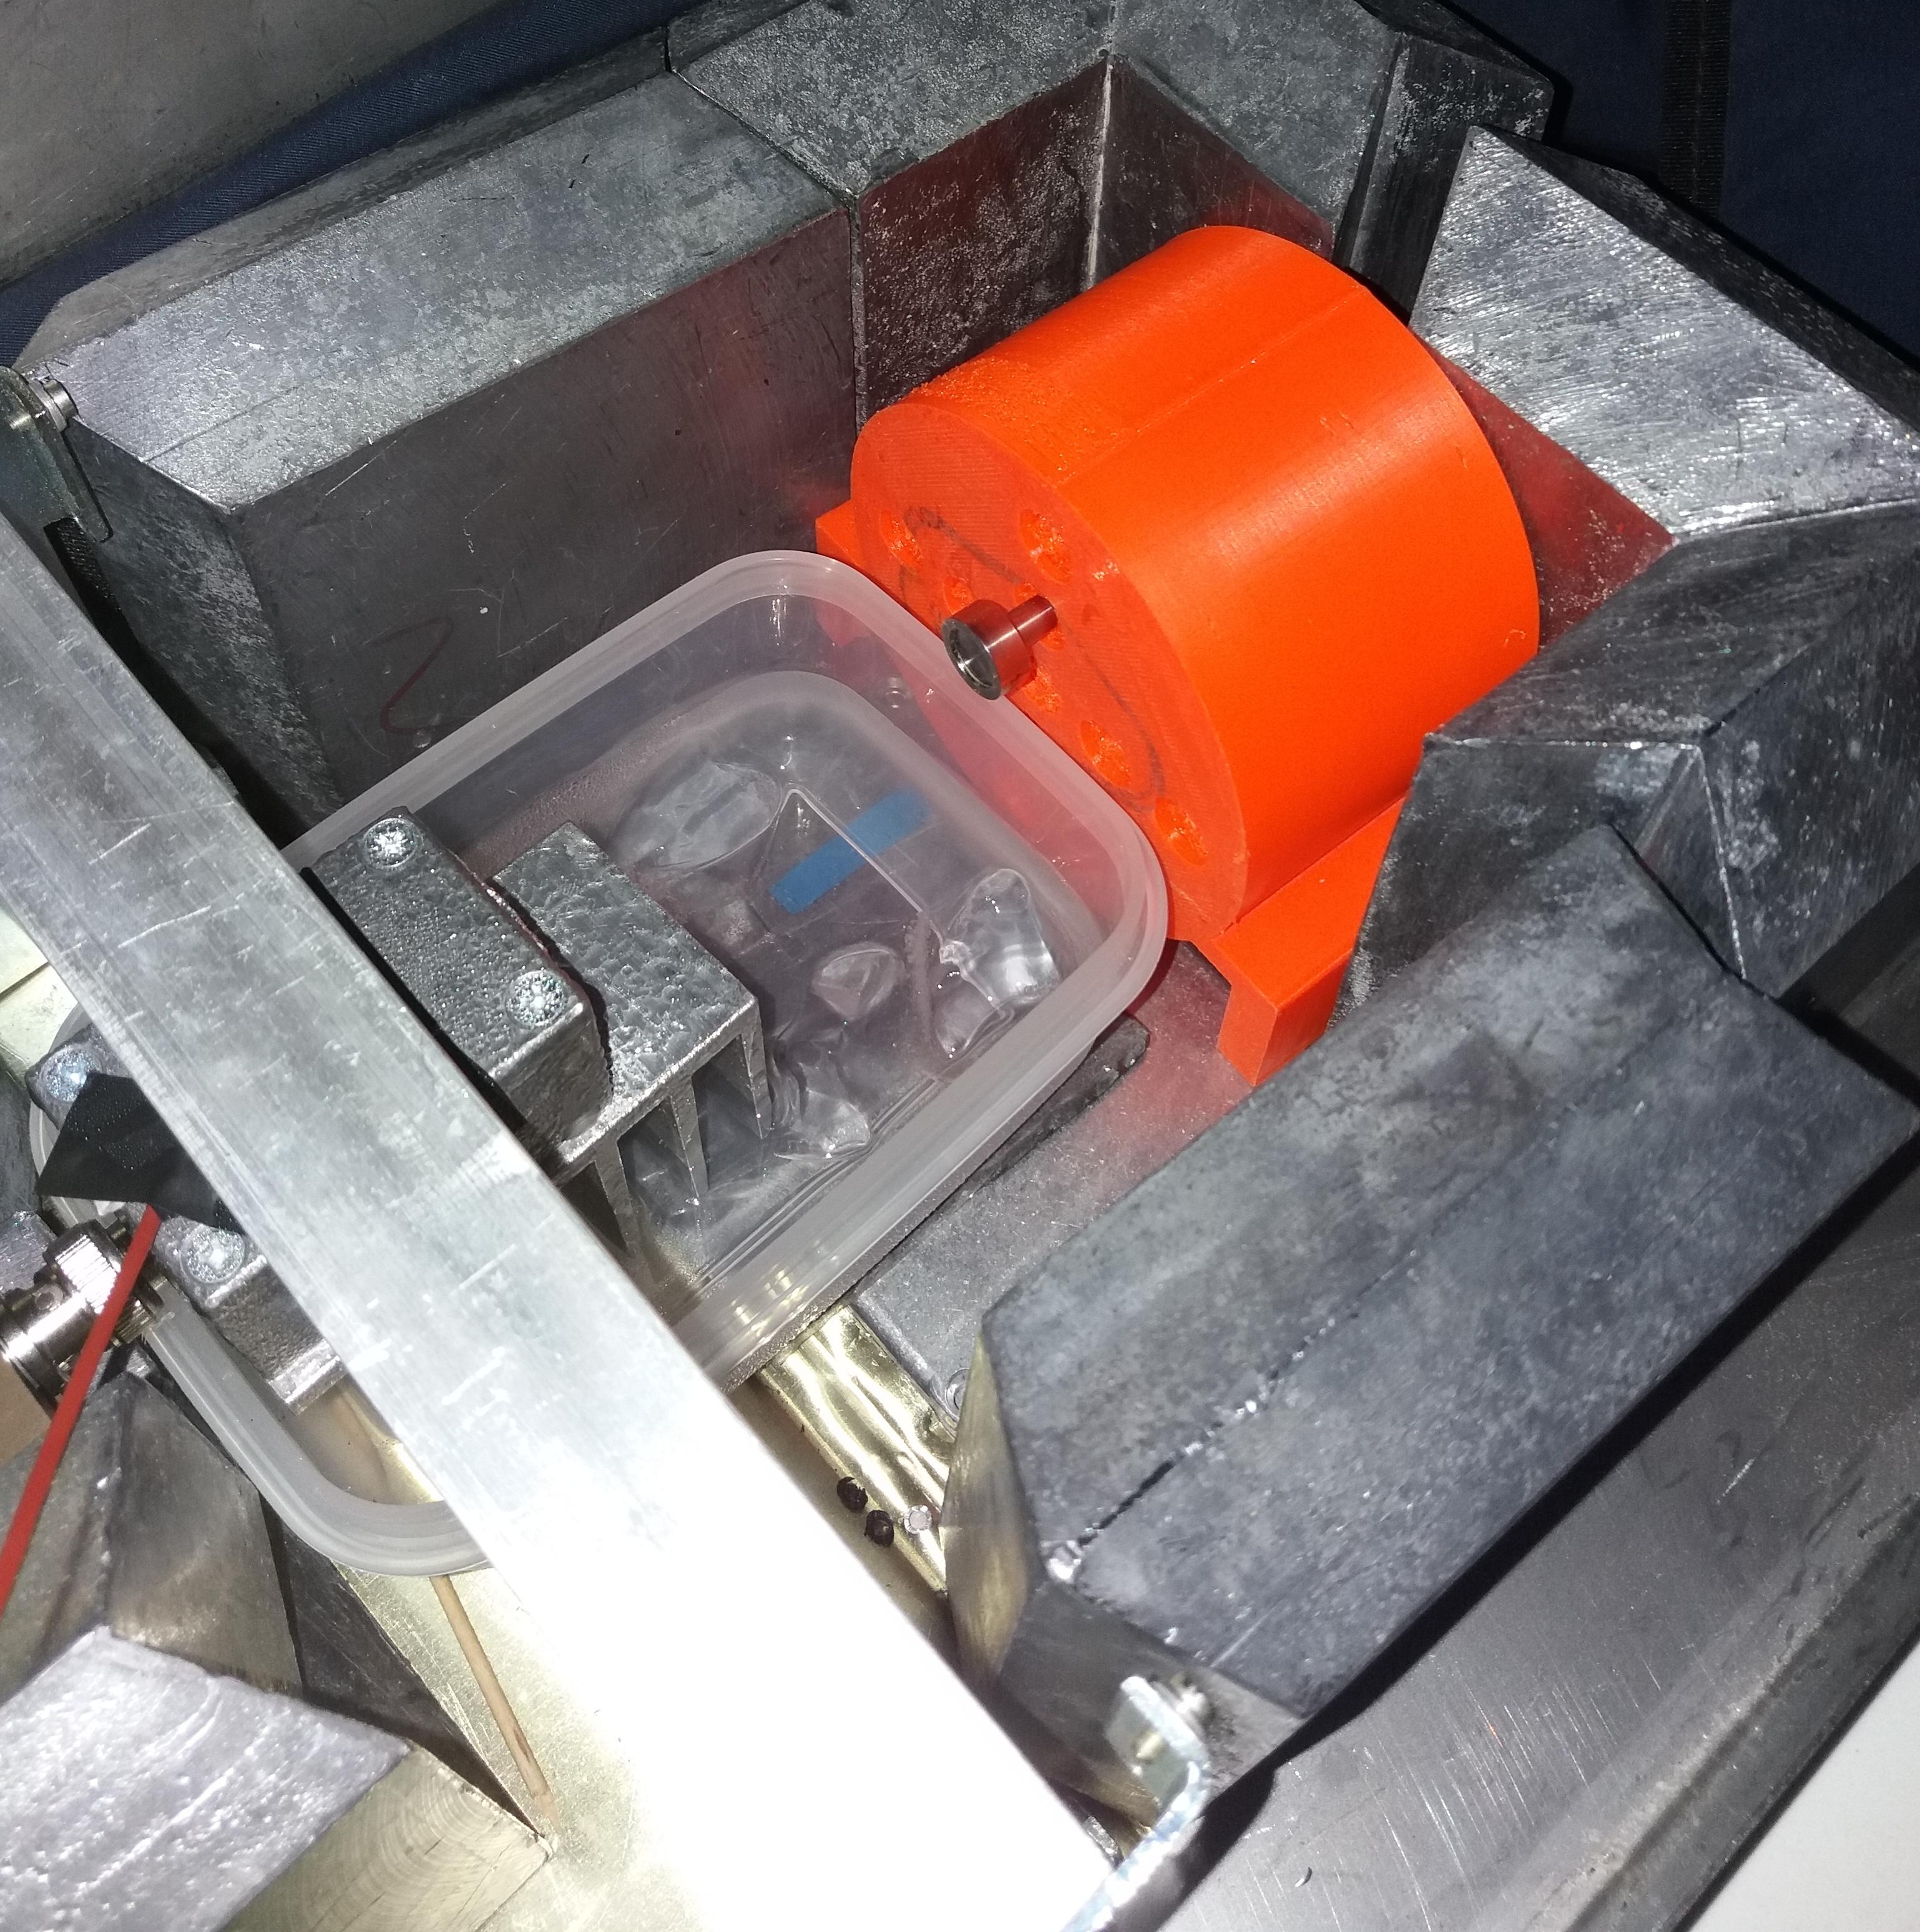
\includegraphics[scale=0.09, angle = 0]{./pictures/chlazeniLedem.jpg}
 \caption{Example of $^{57}$Co spectra from poorly shielded detector setup and from sufficiently shielded detector.}
 \label{notShielded}
 
\end{figure}





\subsection{Thermal noise reduction}
To reduce the thermal noise, the S14605 photodiode was cooled by ice. It was placed in shielding box, which had attached heat sink to the bottom. This heat sink was submerged into the small tub filled with a melting ice (picture \ref{cooler}). The thermal conduction was improved by sticking the photodiode to the of the floor of the shielding box by conduction paste. The photodiode was cooled this way to temperatures around 7-8 $^\circ$C.


\begin{figure}[H]
 \centering
 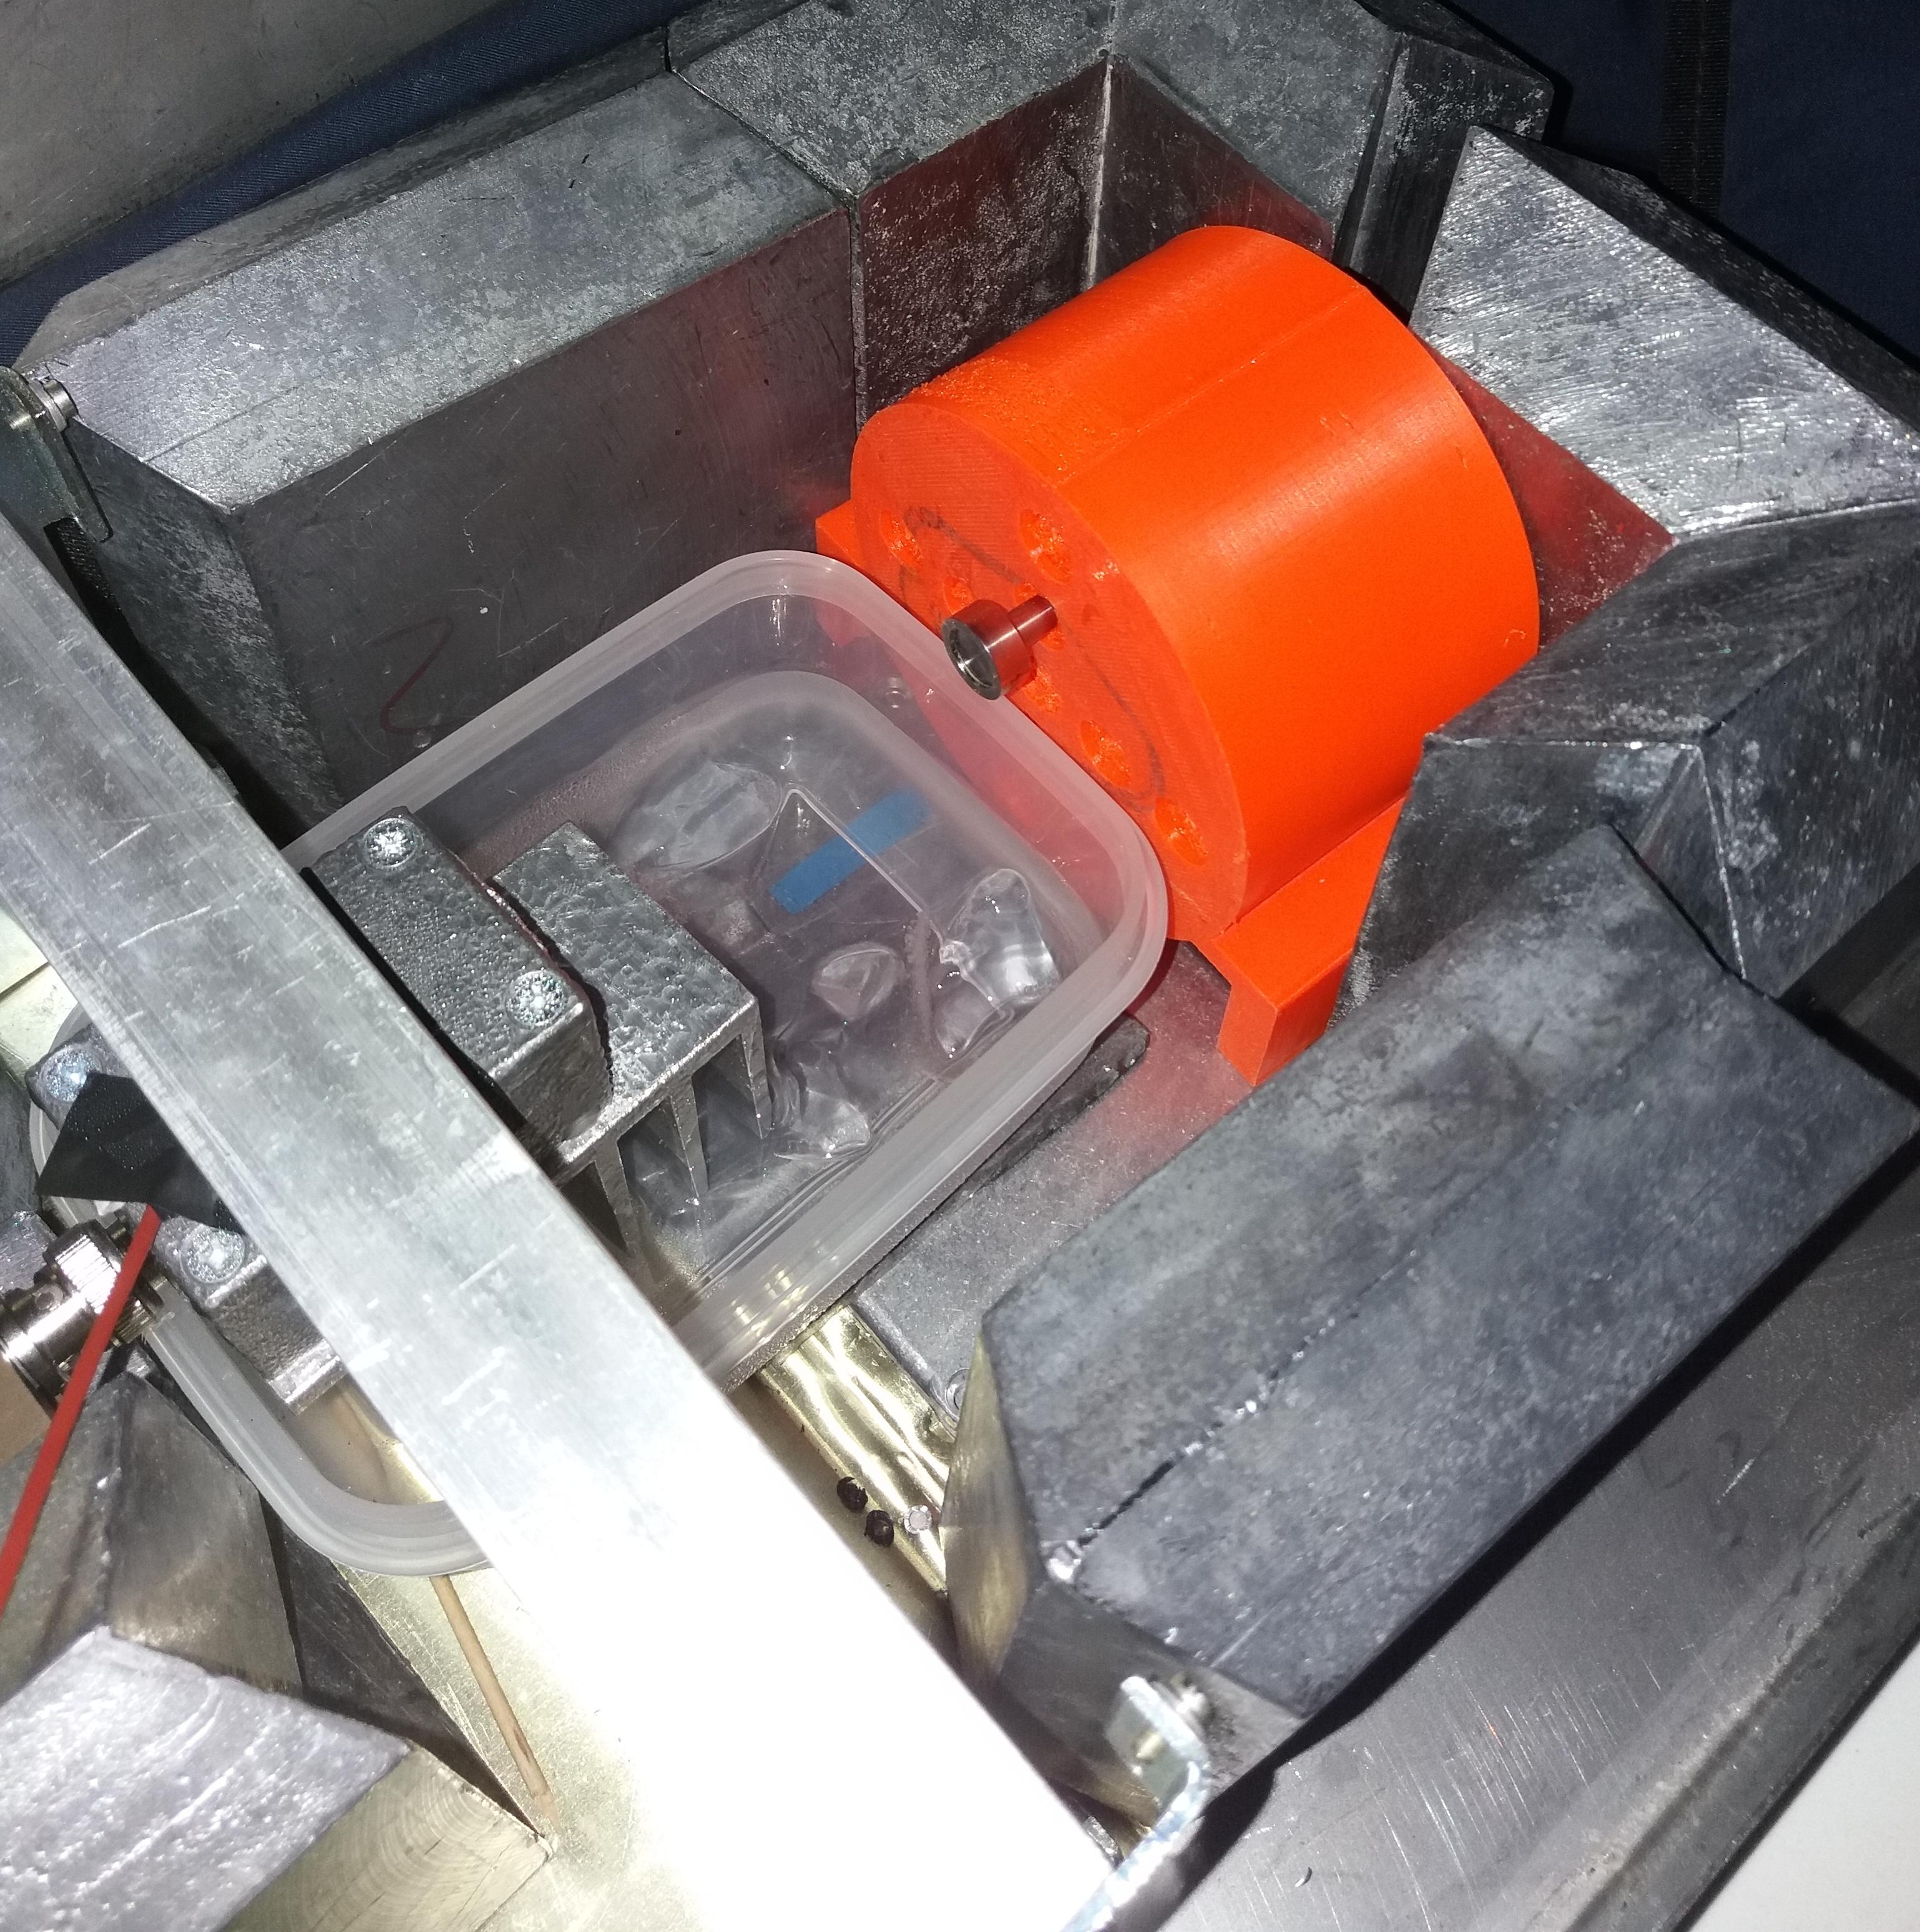
\includegraphics[scale=0.09, angle = 0]{./pictures/chlazeniLedem.jpg}
 \caption{Detector cooled by ice.}
 \label{cooler}
 
\end{figure}



\begin{figure}[H]
 \centering
 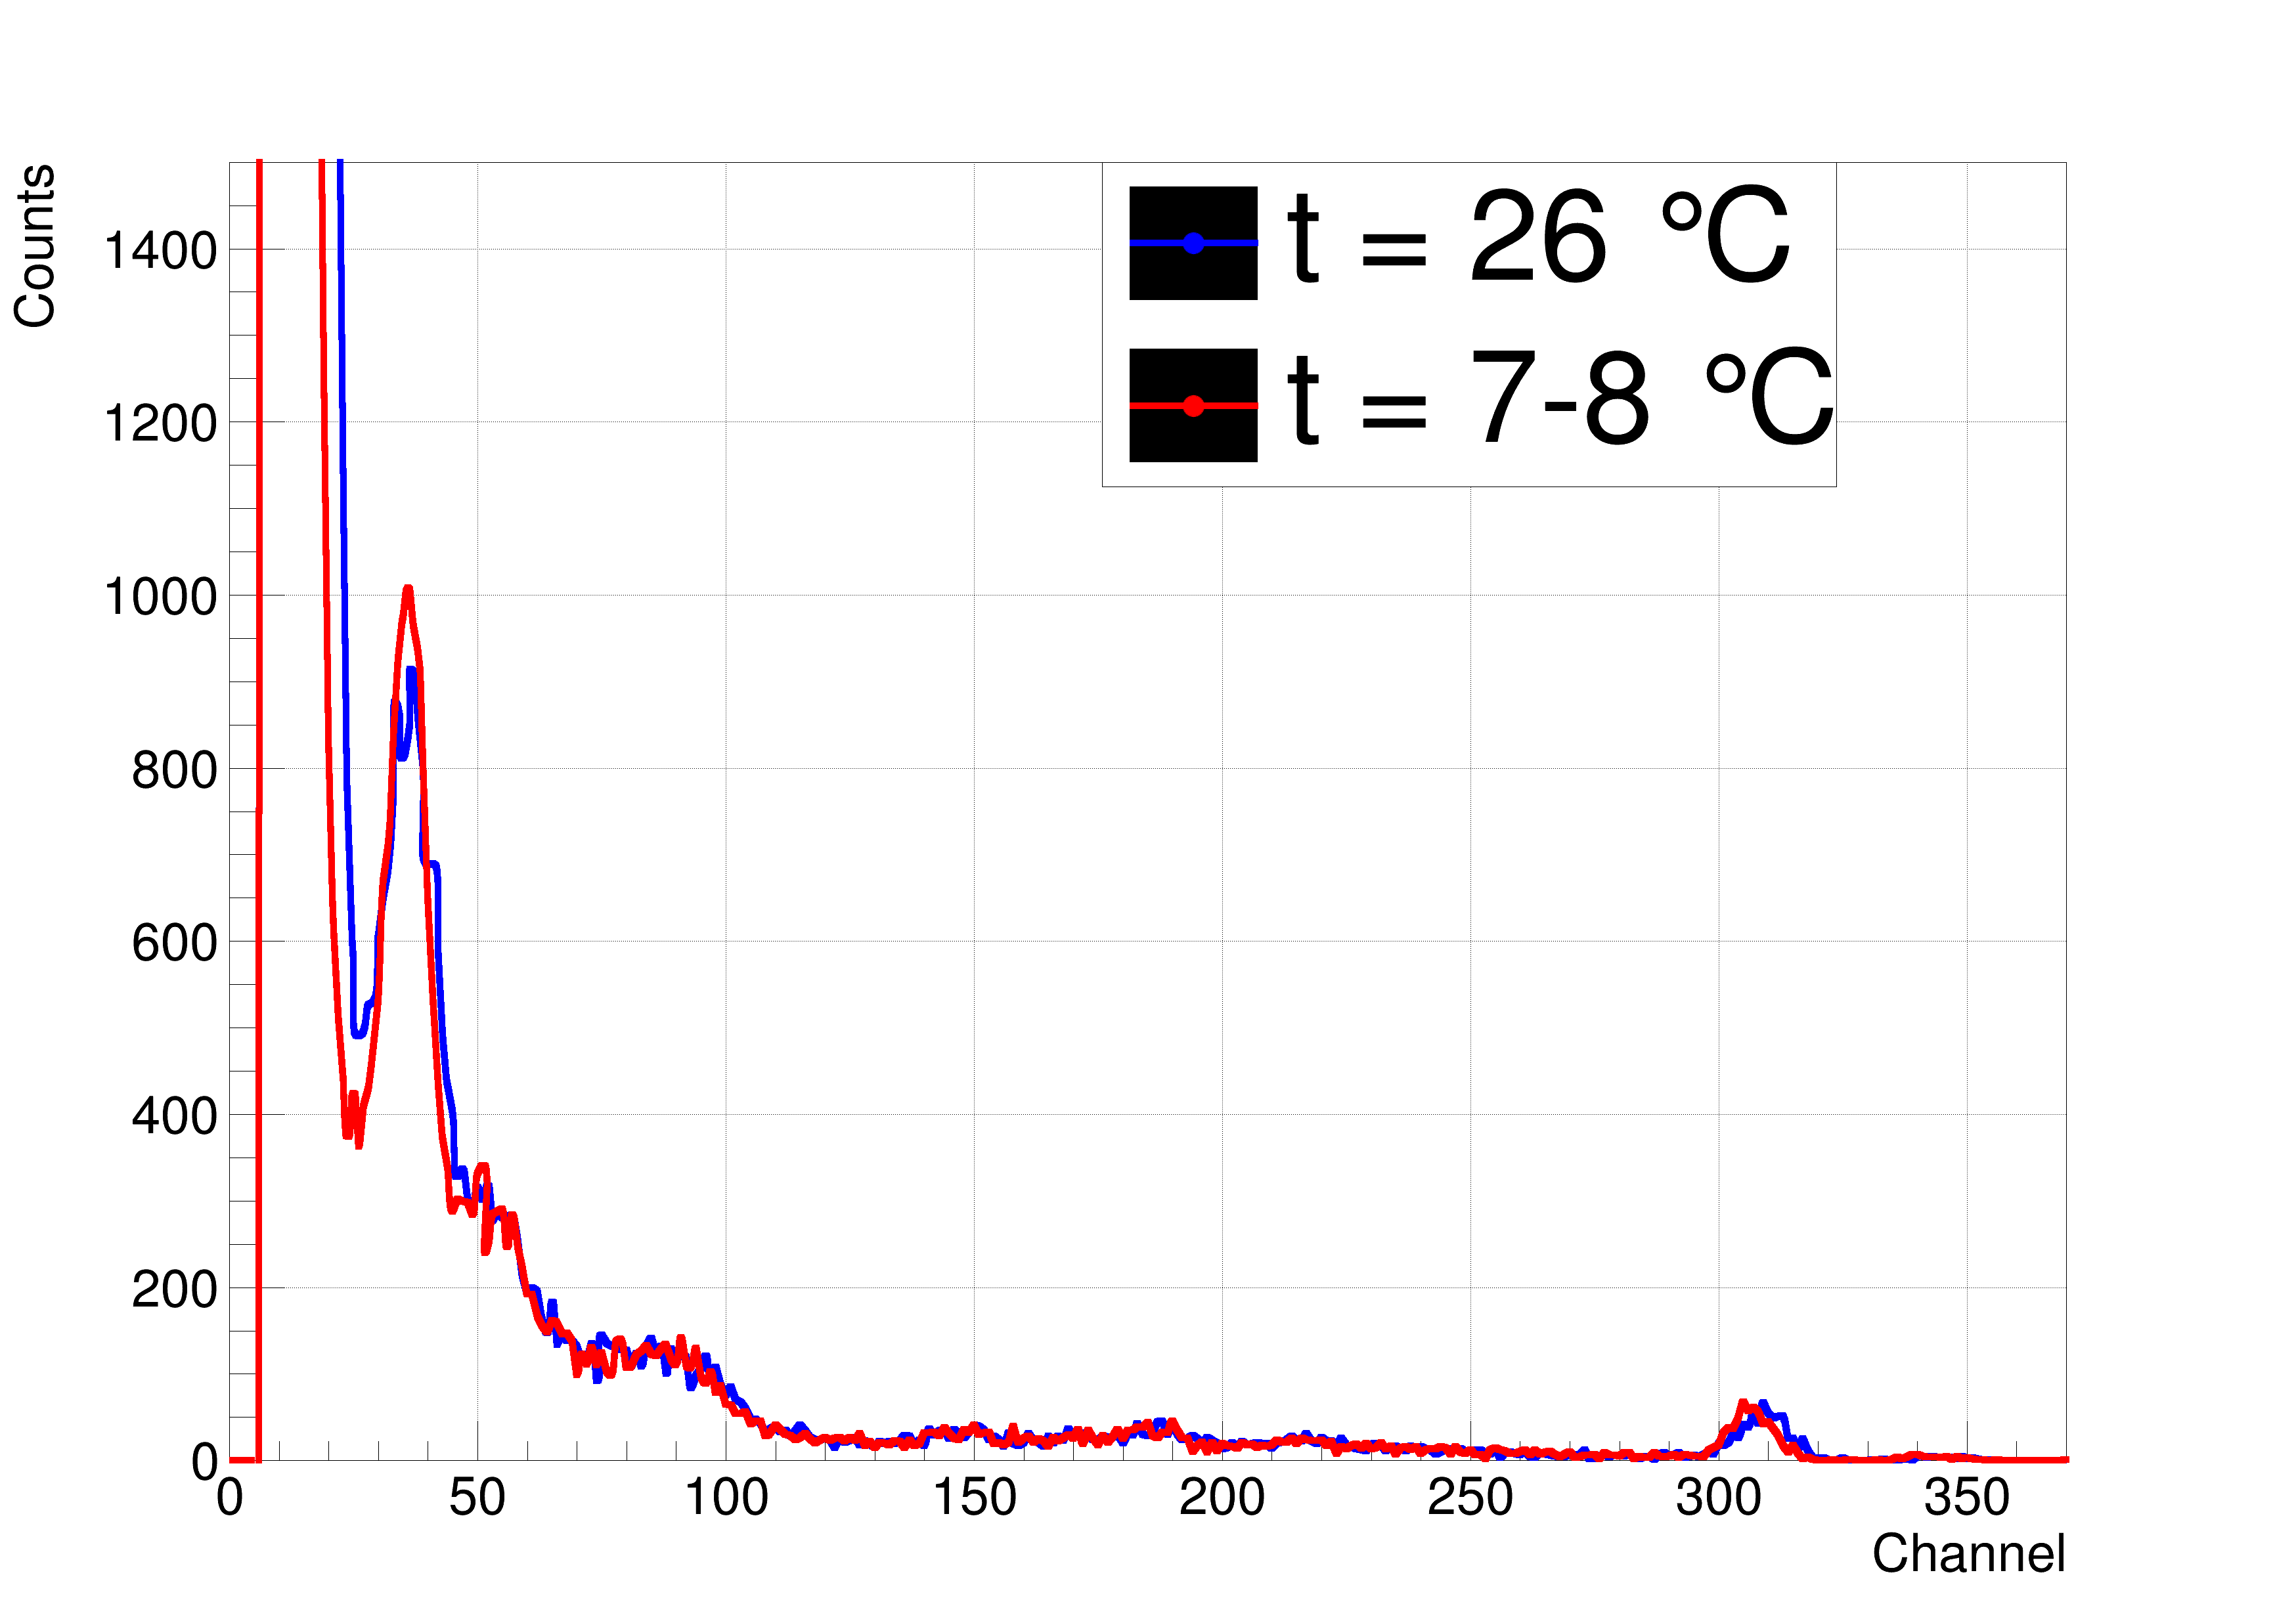
\includegraphics[scale=0.13, angle = 0]{./pictures/TempDiff.png}
 \caption{Measured $^{57}$Co spectra at two different temperatures.}
 \label{coolspectr}
 
\end{figure}








\par
The results show that the cooling improves SNR, but its effect is small when compared to the effect of proper shielding. The cooling is not used in following tests on ORTEC setup.
%It was also tried to use the peltier cooler instead, however, the cooling efficiency was low when compared to the ice.

\section{Detection test of the $^{57}$Co spectra}
The spectra for every photodiode taken for 30 min of real time (MCA allows dead time compensation) with the source's distance 1 cm from the front shielding crate. There is a simple test with a set of filters, which can help us to find out the corresponding energies to the measured peaks:

\begin{itemize}
\item Pb filter: everything should be attenuated.
\item Cu filter: transmitted - 122.1 keV, 136.5 keV not transmitted - 14.4 keV, 6.4 keV.
\item Al filter: transmitted - 122.1 keV, 136.5 keV, 14.4 keV not transmitted - 6.4 keV.
\end{itemize}

The analysed spectre is analysed by peak finder program to find the characteristic energy components. By filter test it can be determined which peak corresponds to 14.4 keV (Cu - attenuated, Al - not attenuated). The channel position of 14.4 keV is then used to recalculate the other peak's channel positions to energies.
\par
The Compton edge caused by interaction of 122.1 keV photons inside the detector can be expected. The equation \ref{compton} estimates the position to be around 39.5 keV. 

\subsection{S14605 test}
From the S14605 capacity graph \ref{datS14605} can be deduced optimal voltage - we decided to set it to 50 V. It was observed that any further increase of voltage do not improves the SNR.


\begin{figure}[H]
 \centering
 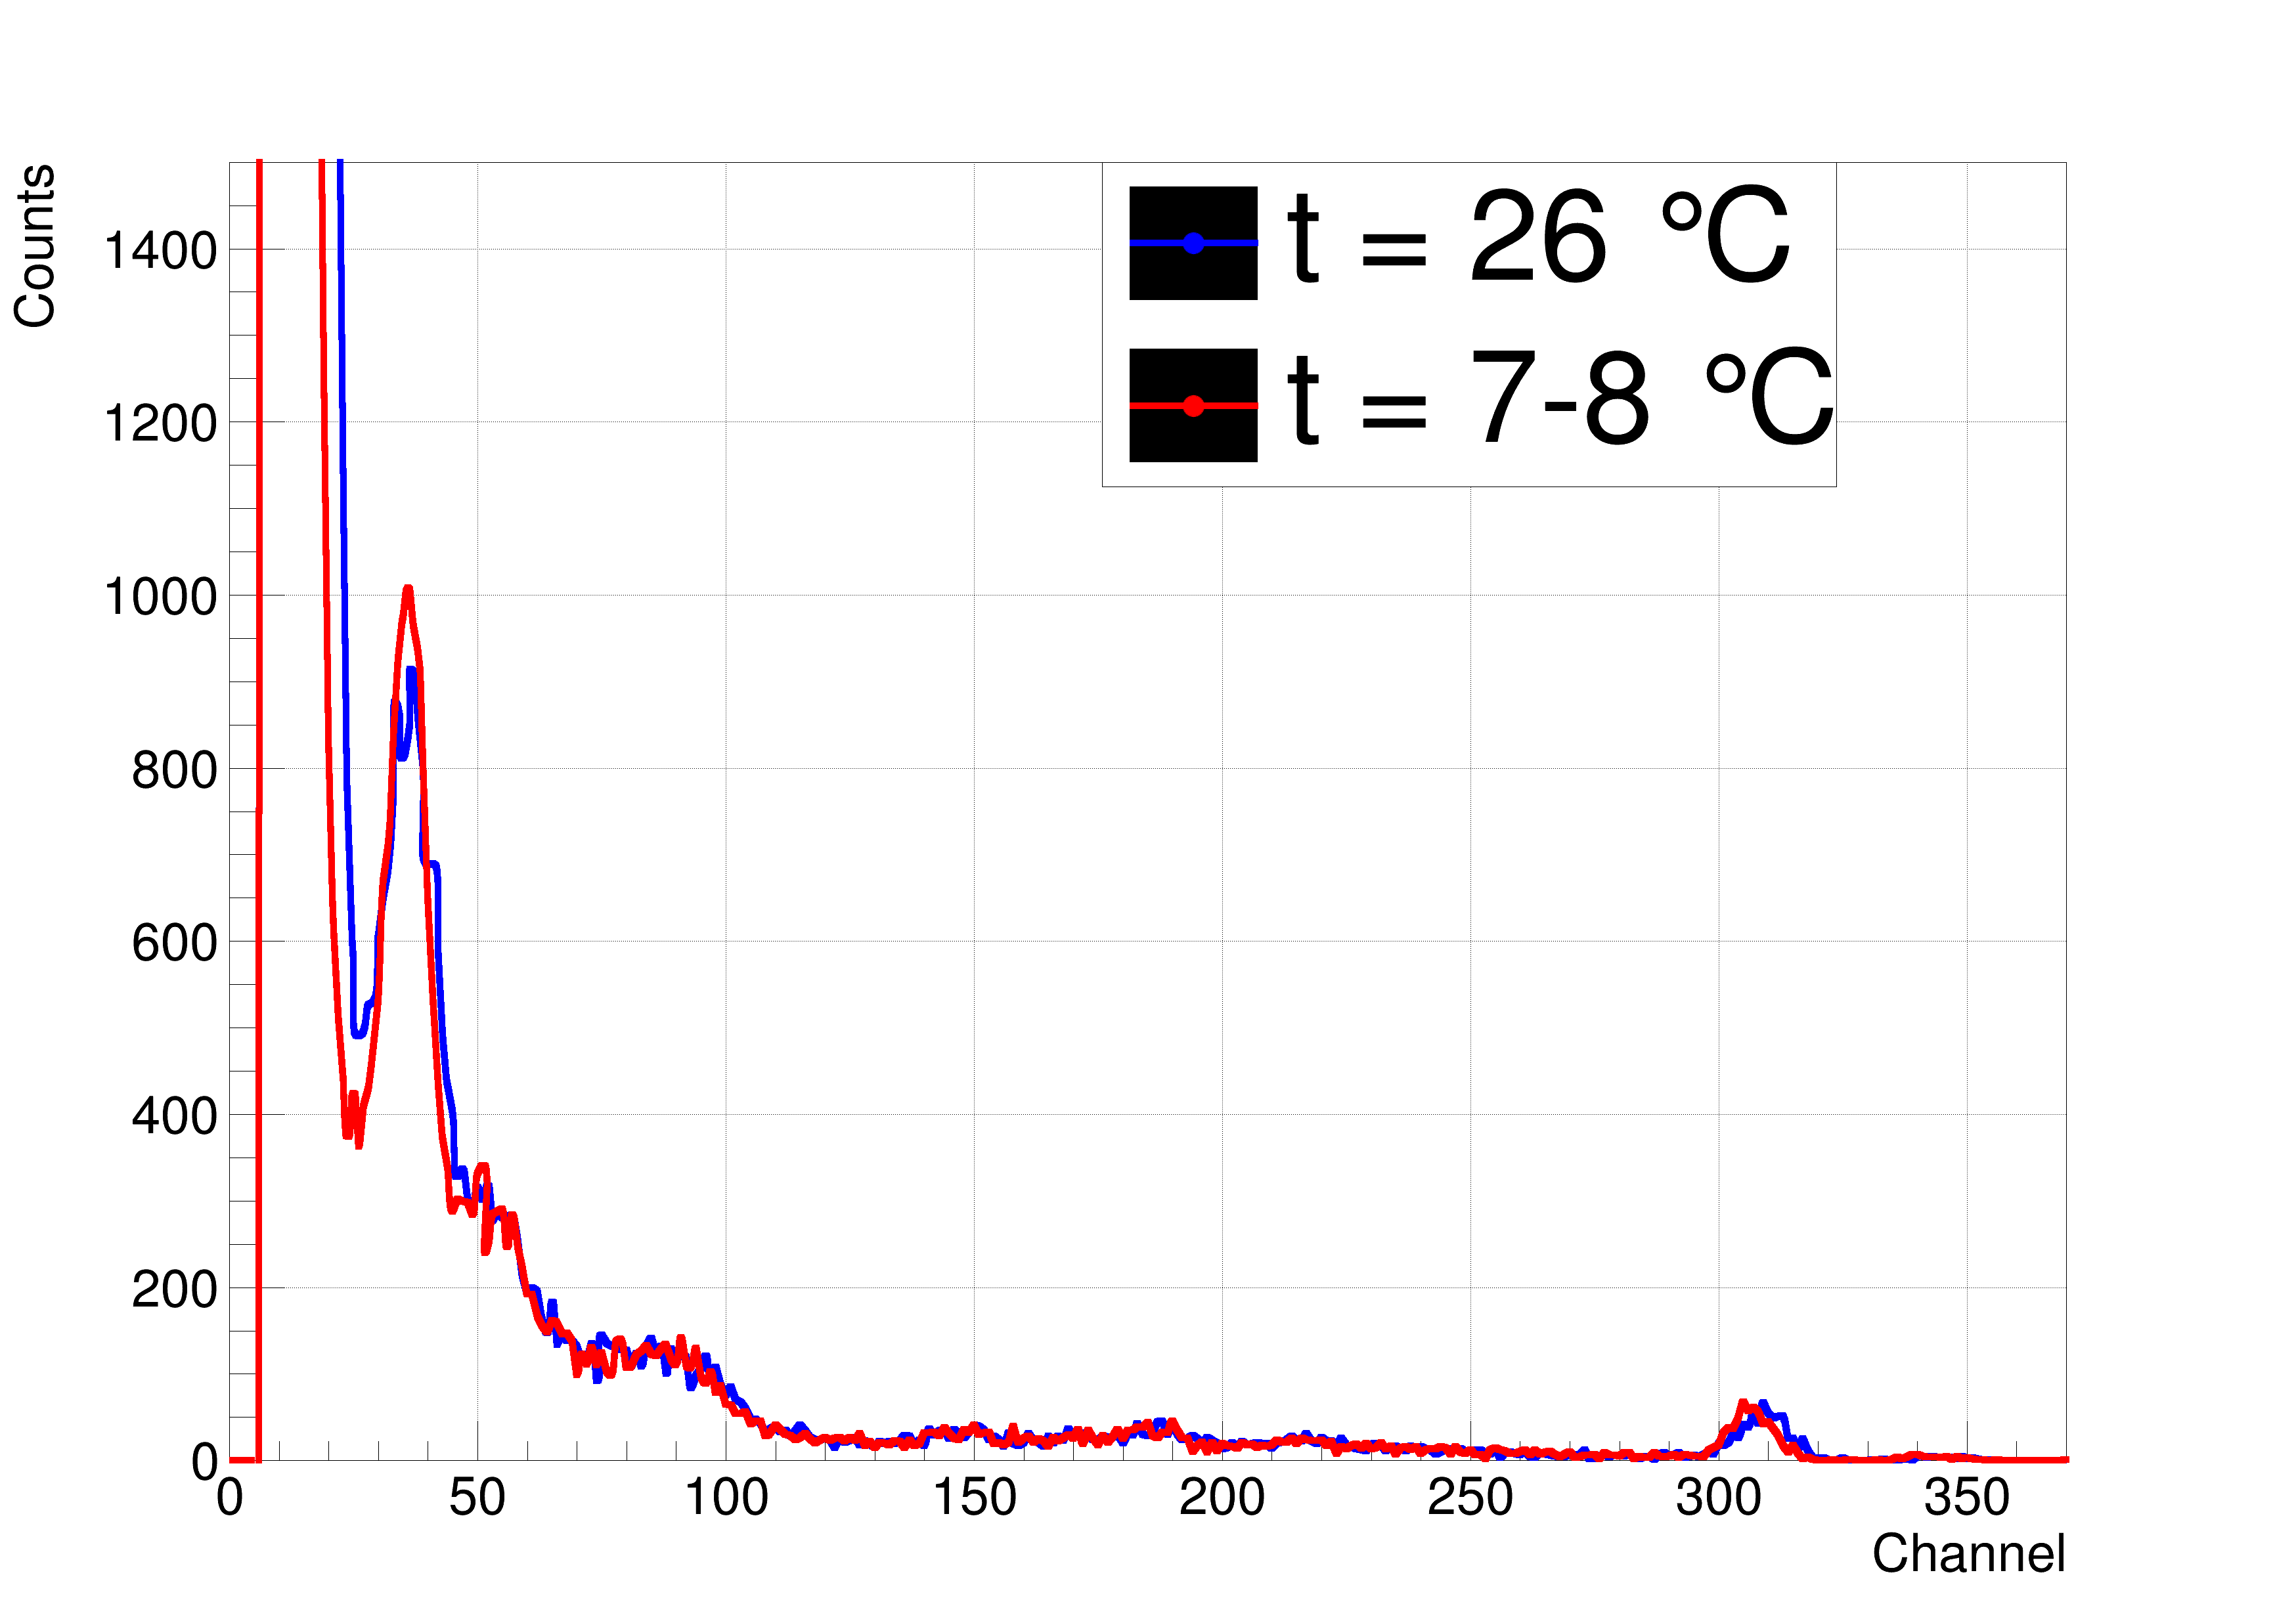
\includegraphics[scale=0.13, angle = 0]{./pictures/TempDiff.png}
 \caption{S14605 spectra with founded energy peaks (green lines) and estimated compton edge (red line).}
 \label{S14605 spectra}
 
\end{figure}


\subsection{BPW34 test}


\begin{figure}[H]
 \centering
 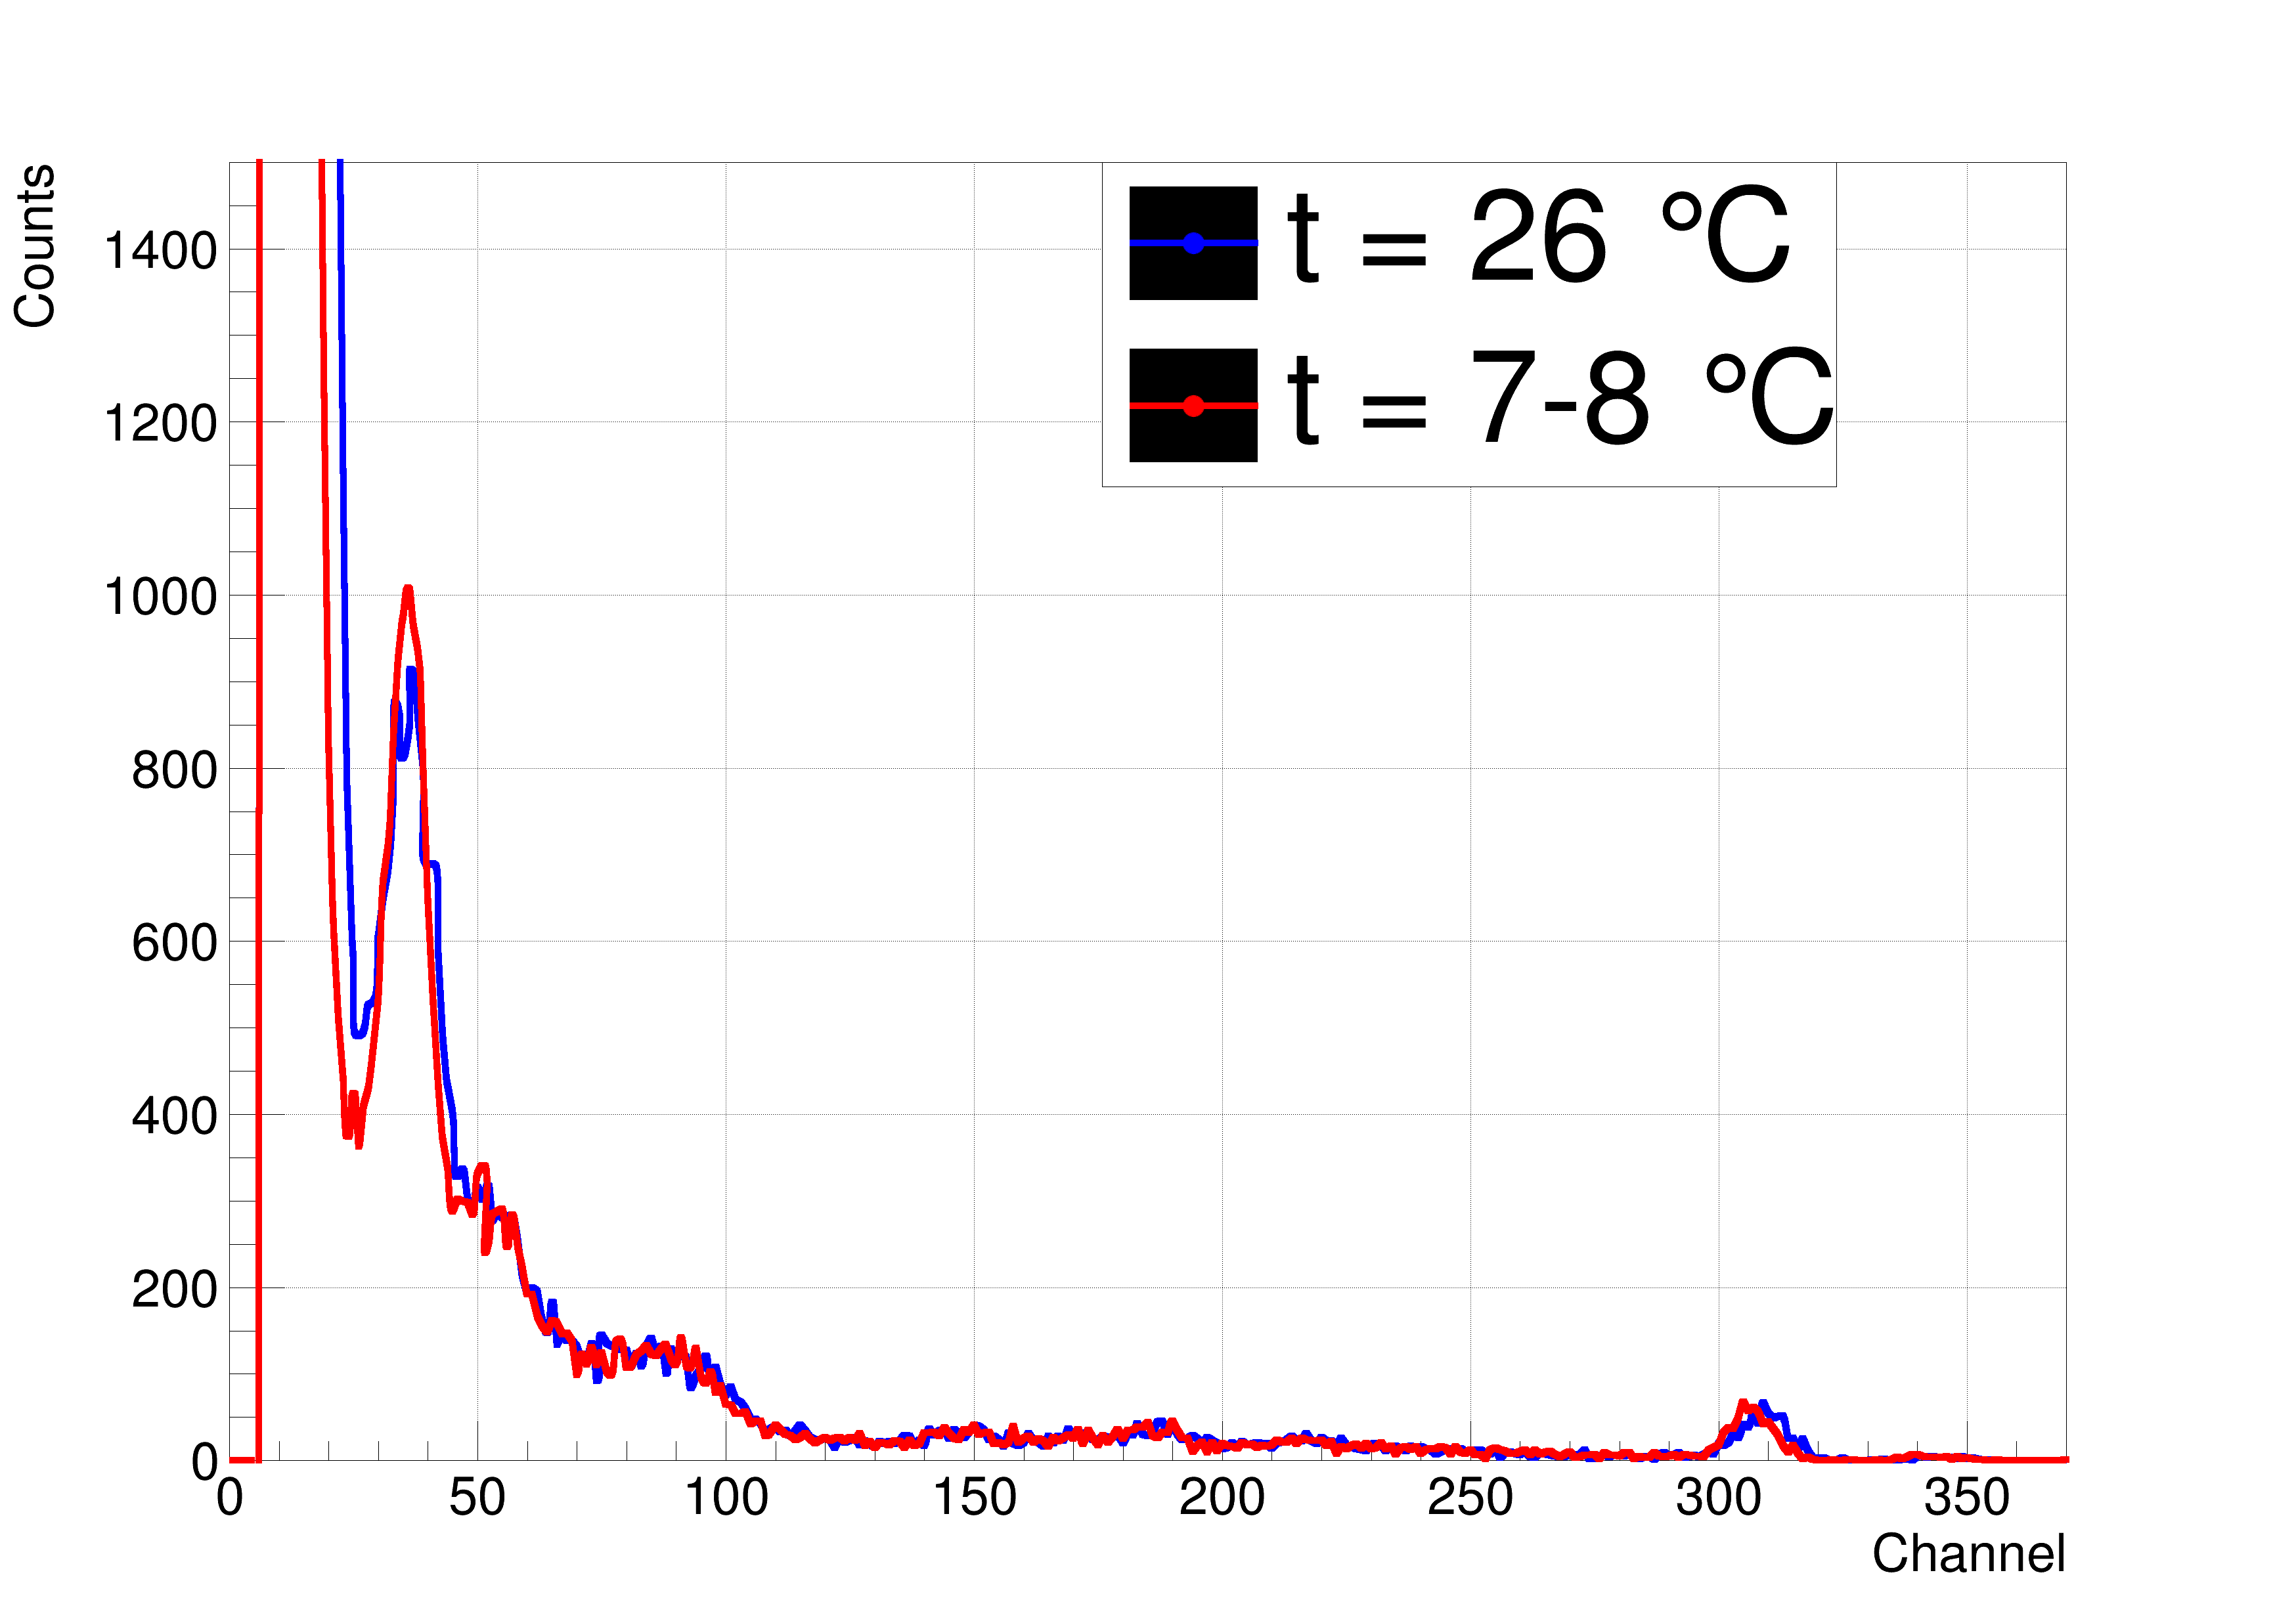
\includegraphics[scale=0.13, angle = 0]{./pictures/TempDiff.png}
  \caption{BPW34 spectra with founded energy peaks (green lines) and estimated compton edge (red line).}
 \label{BPW34 spectra}
 
\end{figure}


It is surprising that this cheap photodiode is capable of capturing gamma rays. The efficiency is lower than S14605 about .
\subsection{OPF430 test}
OPF430 was operated on 20 V. There was a problem with the very low detection efficiency, so the source had to be put into the shielding box right before the photodiode.

\begin{figure}[H]
 \centering
 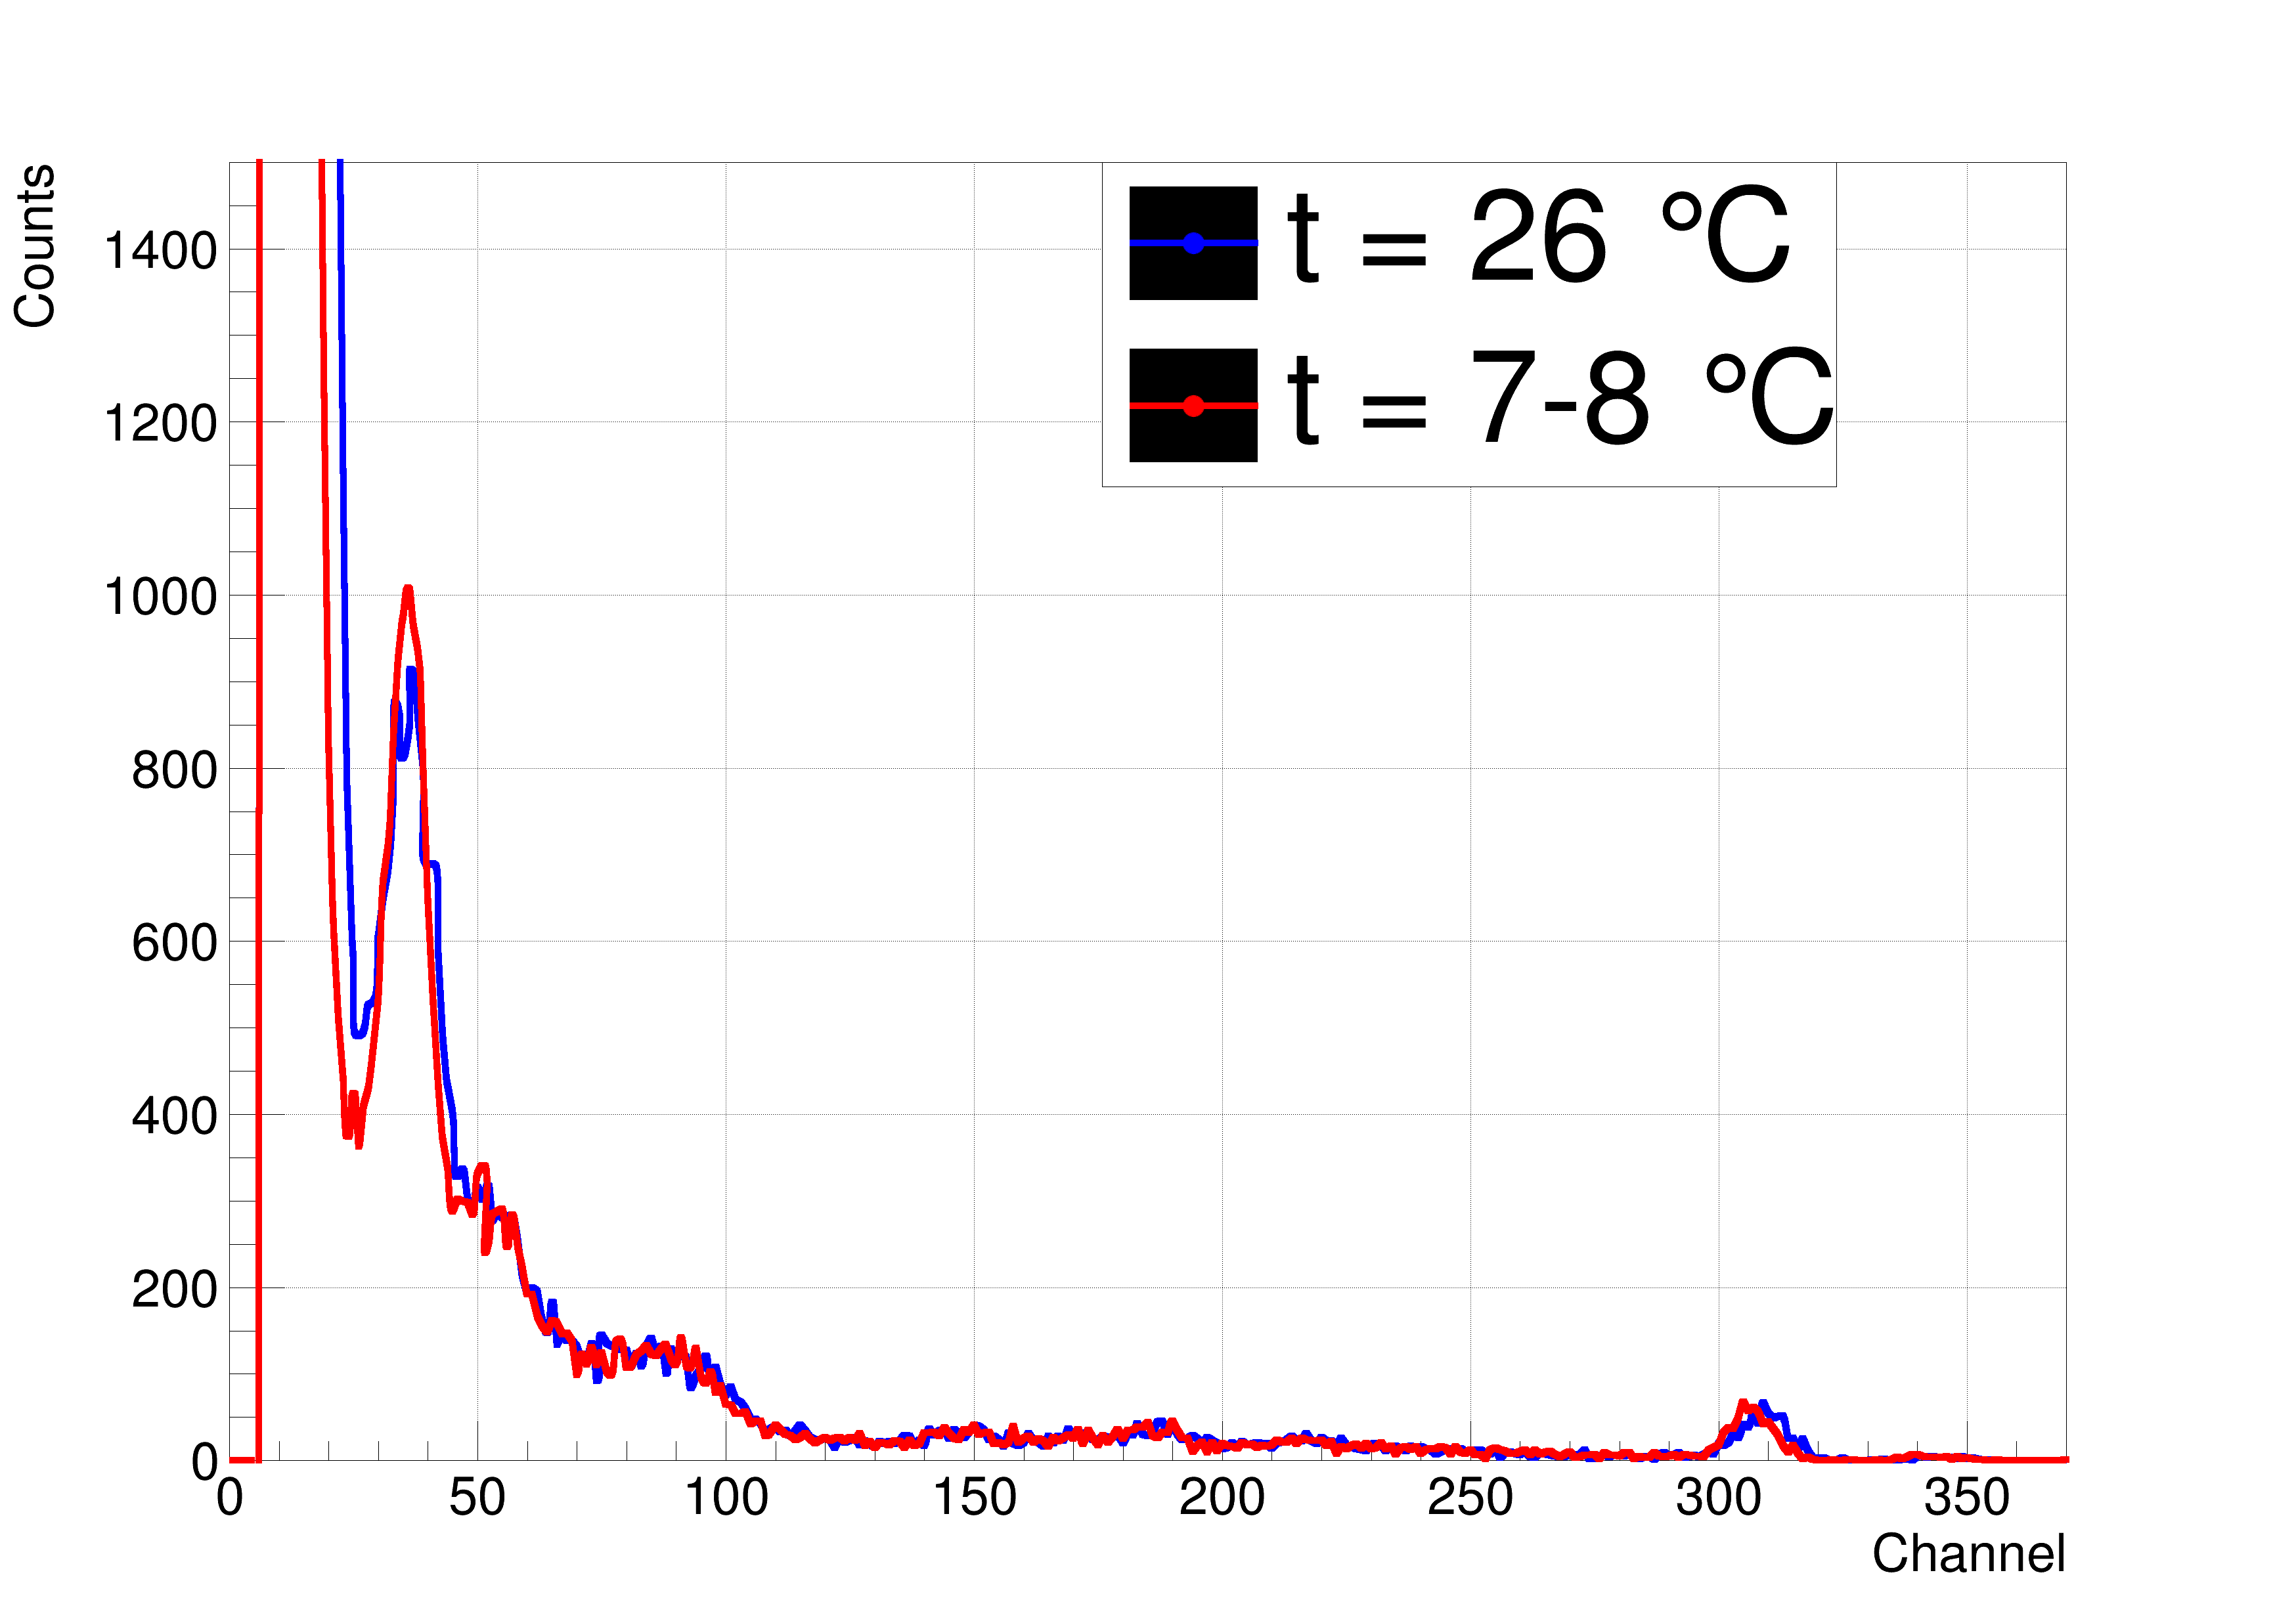
\includegraphics[scale=0.13, angle = 0]{./pictures/TempDiff.png}
 \caption{OPF430 spectra with founded energy peaks (green lines) and estimated compton edge (red line).}
 \label{OPF430 spectra}
 
\end{figure}

It can be seen that the count rates are still much lower that they were measured at previous photodiodes. This is probably due to the fact, that the surface of detector is very small.
The conclusion is that OPF430 is capable of capturing the low-energy gamma rays, however, the efficiency is so bad that it makes it unusable for any real gamma spectroscopy application. 
